%% LaTeX-Beamer template for KIT design
%% by Erik Burger, Christian Hammer
%% title picture by Klaus Krogmann
%%
%% version 2.1
%%
%% mostly compatible to KIT corporate design v2.0
%% http://intranet.kit.edu/gestaltungsrichtlinien.php
%%
%% Problems, bugs and comments to
%% burger@kit.edu

\documentclass[18pt]{beamer}

%% SLIDE FORMAT

% use 'beamerthemekit' for standard 4:3 ratio
% for widescreen slides (16:9), use 'beamerthemekitwide'

\usepackage{templates/beamerthemekit}
% \usepackage{templates/beamerthemekitwide}

%% TITLE PICTURE

% if a custom picture is to be used on the title page, copy it into the 'logos'
% directory, in the line below, replace 'mypicture' with the 
% filename (without extension) and uncomment the following line
% (picture proportions: 63 : 20 for standard, 169 : 40 for wide
% *.eps format if you use latex+dvips+ps2pdf, 
% *.jpg/*.png/*.pdf if you use pdflatex)

%\titleimage{mypicture}

%% TITLE LOGO

% for a custom logo on the front page, copy your file into the 'logos'
% directory, insert the filename in the line below and uncomment it

%\titlelogo{mylogo}

% (*.eps format if you use latex+dvips+ps2pdf,
% *.jpg/*.png/*.pdf if you use pdflatex)

%% TikZ INTEGRATION

% use these packages for PCM symbols and UML classes
% \usepackage{templates/tikzkit}
% \usepackage{templates/tikzuml}

% the presentation starts here
\usepackage{graphicx}
\usepackage{listings}
\usepackage{color}
\usepackage{textcomp}
\definecolor{listinggray}{gray}{0.9}
\definecolor{lbcolor}{rgb}{0.9,0.9,0.9}
\lstset{
	language=Java,
	backgroundcolor=\color{lbcolor},
	tabsize=4,
	rulecolor=\color[rgb]{0.7,0.7,0.7},
  basicstyle=\scriptsize\ttfamily,
  aboveskip=5pt,
  upquote=true,
  columns=fixed,
  showstringspaces=false,
  extendedchars=true,
  breaklines=true,
  frame=lines,
  showtabs=false,
  showspaces=false,
  showstringspaces=false,
  keepspaces=true,
  numbers=left,
  numbersep=5pt,
  numberstyle=\tiny\color[rgb]{0.3,0.3,0.3},
  identifierstyle=\ttfamily\itshape\color[rgb]{0,0,1},
  keywordstyle=\color[rgb]{0.4,0,0.2},
  commentstyle=\color[rgb]{0,0.6,0},
  stringstyle=\color[rgb]{0.627,0.126,0.941},
}
\lstset{literate=%
{Ö}{{\"O}}1 
{Ä}{{\"A}}1 
{Ü}{{\"U}}1 
{ß}{{\ss}}2 
{ü}{{\"u}}1 
{ä}{{\"a}}1 
{ö}{{\"o}}1
}
\usepackage[utf8]{inputenc}
\setbeamercovered{invisible}


\usepackage[utf8]{inputenc}
\usepackage{stmaryrd}
\setbeamercovered{covered}

\title[Prog Tut Nr. 11]{Tutorium Programmieren}
\subtitle{Tut Nr.11: Exceptions, java.util}
\author{Michael Friedrich}
\date{21. / 23.11.2013}

\institute{Institut f\"ur theoretische Informatik}
% Bibliography

\usepackage[citestyle=authoryear,bibstyle=numeric,hyperref,backend=biber]{biblatex}
\addbibresource{templates/example.bib}
\bibhang1em

\begin{document}

% change the following line to "ngerman" for German style date and logos
\selectlanguage{ngerman}

%title page
\begin{frame}
	\titlepage
\end{frame}

%table of contents
\begin{frame}{Outline/Gliederung}
  \tableofcontents
\end{frame}

\section{Exceptions}
\begin{frame}{Fehlerbehandlung}
Wichtig bei:
\begin{itemize}
	\item Öffnen einer Datei, welche nicht existiert
  \item Zugriff auf Array-Element mit ungültigem Index
  \item Division durch Null
  \item ...
\end{itemize}
\pause
\textbf{Probleme:}
\begin{itemize}
	\item Fehler abfangen, weiterleiten, behandeln?
  \item Wie Programmfluss dadurch nicht stören?
\end{itemize}
\end{frame}

\subsection{generelle Fehlerbehandlung}
\begin{frame}[fragile]{Fehlerbehandlung}
	\textbf{Eine Möglichkeit:} Prüfen mittels if-Abfragen
  \begin{lstlisting}
public int positivMultiply(int x, int y) {
  if ((x>0 && y<0) || (x<0 && y>0)) {
    System.out.println("Fehler: ein Argument ist negativ");
    return -1;
  } else {
    return x*y;
  }
}
  \end{lstlisting}
  \pause
  \textbf{Funktioniert, aber:}
  \begin{itemize}
    \item Stört Kontrollfluss
    \item evtl. Ausgaben, wo man sie nicht haben will bzw. sollte!
    \item[] $\Rightarrow$ Vermischung von Logik und Fehlerbehandlung
  \end{itemize}
\end{frame}

\begin{frame}{Exceptions}
	\begin{block}{Exceptions}
    \begin{itemize}
      \item Werden in Fehlersituationen zur Laufzeit ausgelöst ("`geworfen"')
      \item Können in einem übergeordneten Block abgefangen und behandelt werden
      \item Unterbrechen den Kontrollfluss
    \end{itemize}
  \end{block}
  \textbf{Vorteile:}
  \begin{itemize}
    \item[+] Fehler muss nicht lokal behandelt werden, sondern kann weitergereicht werden
    \item[+] saubere Trennung von Logik und Fehlerbehandlung
  \end{itemize}
\end{frame}

\begin{frame}{Exceptions}
	\begin{itemize}
    \item Sind Objekte (\lstinline$Exception$ und Unterklassen)
    \item[] $\Rightarrow$ werden mit \lstinline$new$ erzeugt
    \pause
    \item werden mit \lstinline$throw$ geworfen
    \pause
    \item Methode, welche den Fehler erzeugt (wirft), wird mit \lstinline$throws$ gekennzeichnet
    \item[] \lstinline$public void methode(..) throws IllegalArgumentException$
    \pause
    \item Wird die Exception nicht in der Methode selbst gecatched, so wird sie an die aufrufende Methode weitergeleitet
    \pause
    \item Viele Exceptions in Java-API vorhanden, eigene sind möglich
    \item Java-Doc dokumentation mittels \lstinline$@throws$
  \end{itemize}
\end{frame}

\begin{frame}[fragile]{Exceptions: Vererbungshierarchie}
\begin{figure}[ht]
	\centering
  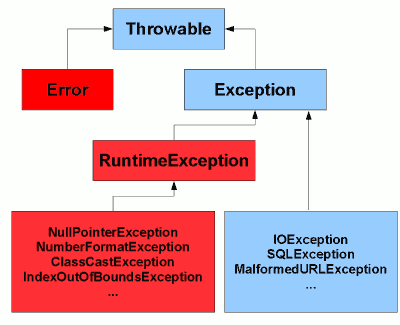
\includegraphics[width=0.7\textwidth]{ExceptionHierarchy.png}
\end{figure}
\end{frame}

\begin{frame}[fragile]{Exceptions: Verwendung}
	\begin{lstlisting}
public int positivMultiply(int x, int y) throws IllegalArgumentException {
  if ((x>0 && y<0) || (x<0 && y>0)) {
    throw new IllegalArgumentException();
  }
  return x * y;
}
  \end{lstlisting}
  \pause
  An \textbf{anderer (aufrufender) Stelle}, wo der Fehler behandelt werden soll:
  \begin{lstlisting}
  try {
    int z = positivMultiply(x,y);
  } catch (IllegalArgumentException e) {
    System.out.println("Fehler: ein Argument ist negativ");
  }
  \end{lstlisting}
\end{frame}

\subsection{try-catch-finally}
\begin{frame}[fragile]{For when you just Gotta Catch 'Em All}
	\begin{figure}%
  
\includegraphics[width=0.5\columnwidth]{pokemon.jpeg}%
  \end{figure}
  \begin{lstlisting}
  try {
    ...
  } catch (Exception e) {
    // Gotcha!
  }
  \end{lstlisting}
\end{frame}

\subsection{Exceptions vs Errors}
\begin{frame}[fragile]{Exceptions vs Errors}
	\begin{block}{RuntimeException}
    \begin{itemize}
      \item Programmierfehler, der zur Laufzeit festgestellt wird, teilweise behandelbar
      \item \lstinline$NullPointerException$, \lstinline$ArrayIndexOutOfBoundsException$
    \end{itemize}
  \end{block}
  \begin{block}{Errors}
    \begin{itemize}
      \item kritische Fehler bei Programmausführung
      \item Nicht behandelbar!
      \item \lstinline$VirtualMachineError$, \lstinline$OutOfMemoryError$
    \end{itemize}
  \end{block}
  \begin{block}{sonstige Exceptions}
    \begin{itemize}
      \item behandelbare Programmfehler, sollte man auf jeden Fall abfangen
    \end{itemize}
  \end{block}
\end{frame}

\begin{frame}[fragile]{Exceptions: finally}
  optionaler Block, welcher auf jeden Fall ausgeführt wird.
	\begin{lstlisting}
try {
  openFile();
} catch (IOException e) {
  printError("File couldn't be read!");
} finally {
  closeFile();
}
  \end{lstlisting}
\end{frame}


\begin{frame}[fragile]{Exceptions}
\begin{lstlisting}
public static void main(String[] args) {
   String input = "";
   BufferedReader buf = new BufferedReader( new InputStreamReader(System.in));
   while(!input.equals("quit")) {  
     try {
       input = buf.readLine();
     } catch (IOException e1) {
       System.out.println("unable to read - shutting down...");
			 input = "quit";
     }
     try {
       int i = Integer.parseInt(input);
     } catch (NumberFormatException e) {
       System.out.println("Eingabe war keine Zahl!");
     }
   }
  System.out.println("shutting down...");
}\end{lstlisting}
\end{frame}

\begin{frame}{Was war bei dem Beispiel wichtig?!}
\pause
\begin{itemize}
	\item Programm stürzt nie unkontrolliert ab \pause
	\item User wird über seine Fehler informiert und kann diese verbessern  \pause
\end{itemize} \pause
Wir als Programmierer müssen unfähigen User (und Kollegen...) entgegen arbeiten. \newline  
Beispiel?  \pause NullPointer abfangen, falsche Werte geliefert, falsche Formattierung...

%%Bild user <--> programmers
\end{frame}

\section{java.util}
\begin{frame}[fragile]{java.util}
Java bietet von sich aus schon sehr viel Funktionalität, z.Bsp LinkedList. \pause
\begin{example}{weitere eingebaute Datenstrukturen} \pause
\begin{itemize}
	\item Collections: ungeordneter Pool an Objekten 
	\begin{itemize}
		\item \lstinline{Collection<Product> products;} \pause
	\end{itemize}
	\item SortedSet: Menge mit totaler Ordnung
	\begin{itemize}
		\item \lstinline{SortedSet<Product> products;} \pause
		\item Product MUSS hier Comparable$<$Product$>$ implementieren \pause
	\end{itemize}
	\item ArrayList: ähnlich LinkedList, aber mit Index
	\begin{itemize}
		\item \lstinline{ArrayList<Product> products;} \pause
	\end{itemize}
	\item Maps: key-value Paare 
	\begin{itemize}
		\item \lstinline{TreeMap<Product, Customer> orders;}
		\item \lstinline{HashMap<Product, Customer> orders;}
	\end{itemize}
\end{itemize}
\end{example}
Nehmt die Hinweise auf dem Übungsblatt als Einstiegspunkt.
\end{frame}

\subsection{Theorie: dynamische Programmierung}
\begin{frame}{dynamische Programmierung}
Was ist das?
	\begin{itemize}
    \item \textbf{kein} Programmierparadigma
    \item sondern:
    \begin{itemize}
      \item Methode zum Lösen von Optimierungsproblemen
      \item benutzt "Divide and Conquer"
      \item wichtig: Gesamtproblem muss ich aus kleineren Teilproblemen zusammensetzen lassen!
      \item speichere Werte kleinerer Probleme in Tabelle ab
    \end{itemize}
    \item[] $\Rightarrow$ Begegnet euch wieder in Algorithmen 1 (2. Semester)
  \end{itemize}
\end{frame}

\begin{frame}{DP: Beispielaufgabe}
	\begin{block}{Levenshtein-Distanz}
    Die \textbf{Levenshtein-Distanz} (auch \textbf{Editierdistanz}) zwischen zwei Zeichenketten ist die minimale Anzahl von \textcolor[rgb]{0,0,1}{Einfüge}-, \textcolor[rgb]{0,0,1}{Lösch-} und \textcolor[rgb]{0,0,1}{Ersetz}-Operationen, um die erste Zeichenkette in die zweite umzuwandeln
  \end{block}
  \pause
  Beispiel: Levenshtein-Distanz von \textcolor[rgb]{0,0.58,0}{"`Tier"'} und \textcolor[rgb]{0,0.58,0}{"`Tor"'}
  \begin{enumerate}
    \item \textcolor[rgb]{0,0.58,0}{"`Tier"'}
    \item \textcolor[rgb]{0,0.58,0}{"`Toer"'} (Ersetze i durch o)
    \item \textcolor[rgb]{0,0.58,0}{"`Tor"'} (Lösche e)
  \end{enumerate}
  \pause
  elegant zu lösen mittels dynamischer Programmierung!
\end{frame}

\begin{frame}{DP: Beispielaufgabe}
	\textbf{Eingabe:} Zeichenketten $u$ und $v$\\
  \textbf{Matrixeinträge} $D_{i,j}$ speichern die Distanz der Präfixe $u_{0,i}$ und $v_{0,j}$.\\
  Die Distanz-Werte berechnen sich wie folgt:
  \begin{figure}%
  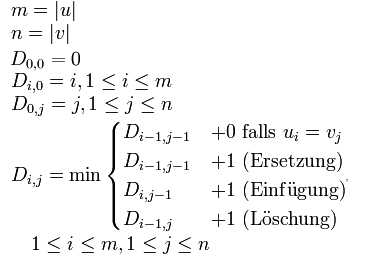
\includegraphics[width=0.6\columnwidth]{distance.png}%
  \end{figure}
\end{frame}

\appendix
\beginbackup

%\begin{frame}[allowframebreaks]{References}
%	\printbibliography
%\end{frame}

\backupend

\end{document}
